\section{APR}
\subsection{What is APR}
Firstly, please read the official description. If you haven't read it, please make sure to read every word carefully, because the importance of APR is equivalent to a small defense. If you fail, you may be expelled.

\url{https://www.liverpool.ac.uk/student-administration/research-students/progression/annual-progress/}

In my understanding, the purpose of APR is
\begin{itemize}
    \item Interview: Pursuing a PhD is not easy, so the university and the school need to understand the problems students encounter and help solve them.
    \item Seminar: Exercise presentation skills and get to know other PhD students.
    \item Progress report: Check student progress, further discover and help solve problems students encounter. At the same time, screen out students who are not studying seriously at all.
\end{itemize}

Some students may feel nervous when facing APR for the first time. In fact, as long as you haven't been idling away for the entire year—reading books, reading literature, writing articles, doing surveys, conducting experiments, writing code, etc.—the reviewers will not make things difficult for you and won't fail you. It is said that in 2022, a student in a certain school failed the APR. According to reliable sources, this person almost disappeared from human society, didn't reply to the supervisor at all, and didn't do any work, which is why they failed.

Also, note that another main function of APR is to help everyone solve problems. Therefore, you should boldly expose your problems in the APR and seek help (Chapter \ref{sec.IPAP}).

\subsection{APR Process}
\subsubsection{Preparation Work}
The pre-requisite task for APR is only one, which is to fill in the meeting records at least once a month. For how to fill out the meeting records, refer to Section \ref{sec.meeting_record}.

Then, each year there are two important emails about APR:
\begin{enumerate}
    \item 
        \begin{minipage}{0.3\textwidth}
            The first is an email sent by XJTLU in May, which looks like this, sent to your XJTLU email.
        \end{minipage}
        \begin{minipage}{0.63\textwidth}
            \begin{figure}[H]
                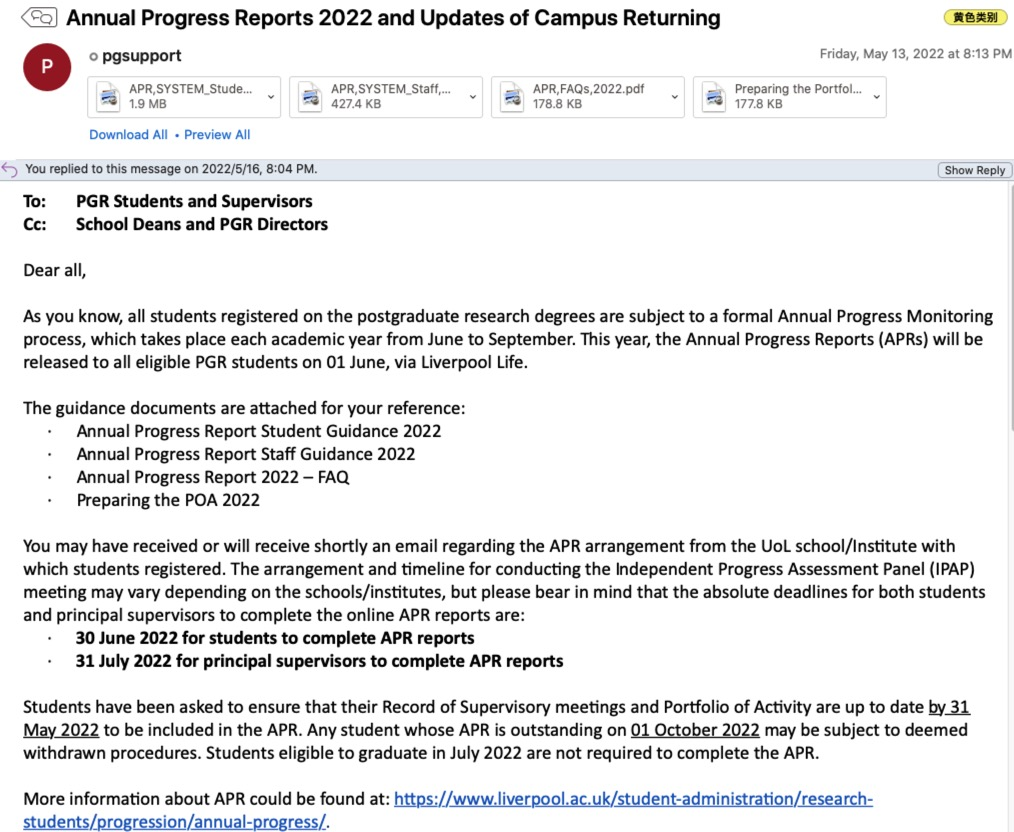
\includegraphics[width=0.95\columnwidth, right]{author-folder/Kai.Wu/APR_email.jpg}
            \end{figure}
        \end{minipage}

    \item 
        \begin{minipage}{0.3\textwidth}
            The second is an email sent by your University of Liverpool school between April and May. For the Mathematics school, it looks like this and is sent to your Liverpool email. Other schools may be different. The time when each school sends the notification also varies greatly, some as early as April, some delayed until the end of May.
        \end{minipage}
        \begin{minipage}{0.63\textwidth}
            \begin{figure}[H]
                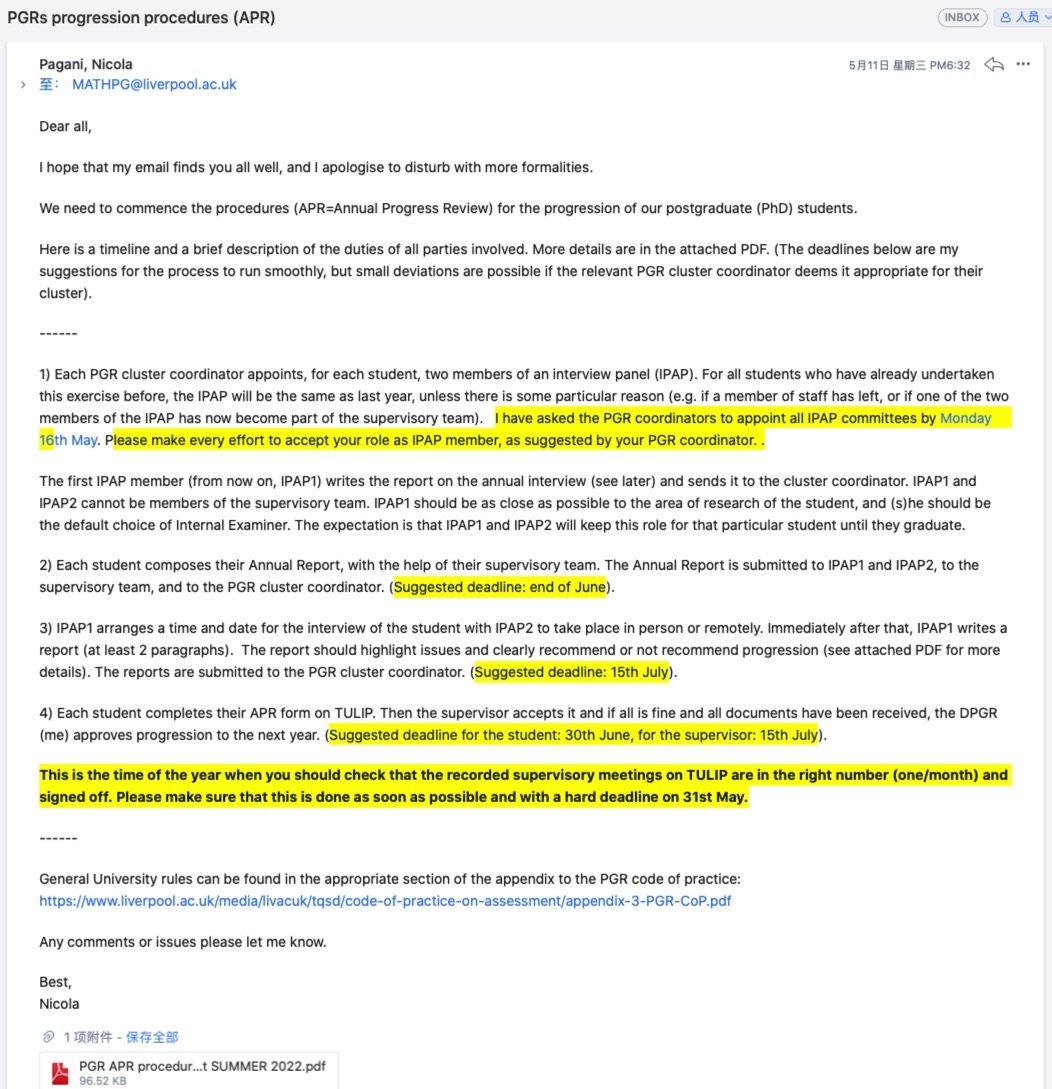
\includegraphics[width=0.95\columnwidth, right]{author-folder/Kai.Wu/APR_liverpool_email.jpg}
            \end{figure}
        \end{minipage}

\end{enumerate}

The APR requirements of each school are slightly different, so around May, please be sure to check your Liverpool email. Read both emails carefully. For students doing APR for the first time, it is recommended to read the two emails and attachments word by word.

The specific content of APR includes the following four parts:

\subsubsection{TULIP Web Form}
What the Liverpool and XJTLU emails refer to as "Your annual progress report has been released" means that you can fill in this green form. The main parts to fill in are:
\begin{enumerate}
    \item SUMMARY OF PROGRESS: Progress report, above 300 words, below 4000 characters (about 600 words).
    \item Seminars and Conference attendance, Library and IT training and all subject-specific training including research methods and experimental techniques. (Recall, the more the better, if you really have none, it's okay.) Seminars, conferences, professional skills training you've attended.
    \item Attendance at careers events and workshops covering Employability and Entrepreneurship and including attendance at any other Professional development workshops. (The more the better.) Career-related activities you have attended.
    \item Training and completion of activities relating to Health and Safety, ethics, grant writing, and similar activities, including Project Management. (The more the better.) Activities not directly related to study but relevant.
    \item Details of your presentations, written publications, teaching and public engagement/impact activities, and related training for these activities. (The more the better.) Presentations, published papers, teaching assistant work you've done.
    \item PERSONAL OR ACADEMIC PROBLEMS: Have there been any problems in the last year which you feel have affected your progress? (Fill in according to the actual situation.) Have you encountered any problems that hindered your studies. You can sincerely raise problems, or appropriately explain, such as "My progress is insufficient because of xxxxx (illness/marriage/poor school network/slow English reading/insufficient ability in certain aspects)."
\end{enumerate}

\begin{figure}[H]
    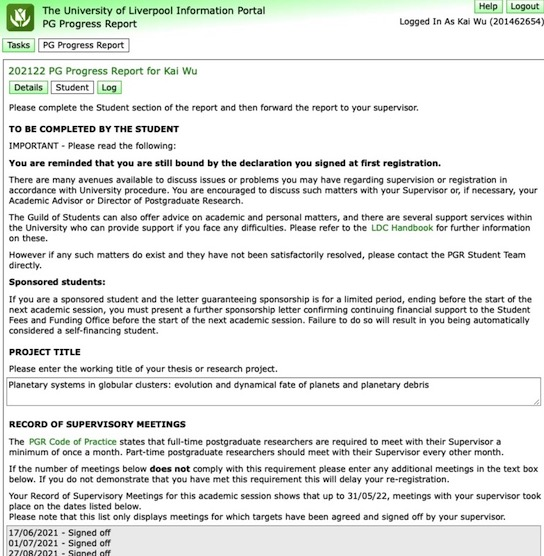
\includegraphics[width=0.7\columnwidth, center]{author-folder/Kai.Wu/TULIP.jpg}
\end{figure}

All students are required to fill in the TULIP form regardless of the school. But the following three parts may have very different requirements for each school, and also partially depend on the University of Liverpool school you belong to. You might want to double-check with your seniors.

\subsubsection{Annual Report (AR)}
In short, write a document about what you've done. There might be word or page requirements. If you really don't know what to write, I personally suggest you can write everything in detail (like a diary), for example, what literature you read and what you gained; what code you wrote or experiments you did. Importantly, what academic activities you've participated in, such as conferences, meetings, and being a teaching assistant, can all be included. In other words, just repeat the content of the TULIP form in the document, basically copy and paste, and if the word count is insufficient, expand the content.

Of course, if there are special requirements, follow them. For example, the Mathematics school requires Year 3 students to submit a Thesis Outline, so you don't need to write a diary.

Please note that this description of the AR part is based on my own experience in the School of Mathematics and Physics. According to other students, many schools have similar requirements, but some schools require much more. According to a chemistry student, they had to write a 30-50 page literature review in the first year, which must be prepared one or two months in advance. New students must consult your seniors or supervisors.

\subsubsection{Annual Seminar}
Generally, all PhD students in a school or department are gathered to do presentations, give each other feedback, and get to know each other. As far as I know, some departments with fewer people skipped this part or merged it into the interview below, turning it into a presentation to two teachers. In any case, you need to prepare a \textbf{PPT} to let others understand your research. You can prepare for a 20-minute presentation plus a 5-minute Q\&A session; some schools may have different requirements, so ask seniors. If you have a lot of research results, you can highlight them; if not, you can present what you've done like a diary to fill the time, making the teachers feel you've done a lot of work.

\subsubsection{IPAP Interview}
\label{sec.IPAP}
The school will find two teachers who are not your supervisors and have no conflict of interest with you to have a face-to-face talk. You may need to prepare a \textbf{PPT} and confidently include your issues in it. All the following problems can be discussed with the IPAP teachers. According to the requirements, the two teachers will do their utmost to help you solve problems:
\begin{itemize}
    \item Equipment problems: School computer malfunctions, such as inconvenient use, lagging, crashes; office environment problems (e.g., air conditioning blowing directly on your head).
    \item Real research problems: You've read too few papers and don't know how to read efficiently; you don't know experimental methods; you have great difficulties in writing; due to non-subjective reasons, you cannot attend many academic meetings (for example, in recent years, every year during APR we complain about various impacts of the pandemic), etc.
    \item Supervisor problems: Your supervisor exploits you, making you work excessively every day, leaving you exhausted; your supervisor makes you do a lot of unrelated work, such as moving house for them, getting takeout, handling reimbursements; your supervisor is very harsh on you, pressuring you, making you highly stressed every day; your supervisor frequently calls, sends messages, or emails outside of work hours and asks you to respond immediately, leaving you no rest; your supervisor takes the first authorship of your paper; your supervisor is often unavailable, not replying to your emails for several days. These problems are serious derelictions of duty by the supervisor. Once encountered, they can cause severe psychological burdens and affect future work efficiency. IPAP is here to address this, so be sure to discuss it clearly with the interviewing teachers.
    \item Emotional and psychological problems: Anxiety, nervousness, insomnia, depressive tendencies (Note: If you feel you are not in a good state, please contact the school's counseling center at \email{counsellingservice@xjtlu.edu.cn} as soon as possible; it's free).
    \item Family pressure: Your family expects you to graduate in 3 years, but you feel too much pressure.
    \item Financial pressure, health problems (serious discomfort that may require you to suspend or take leave to recuperate), any problems that affect your normal PhD work.
\end{itemize}

\vspace{5mm}
Identifying and solving all problems, then starting the next academic year, is the main purpose of APR. If there are any problems that APR cannot conveniently address or solve, please communicate with your supervisor, department head, dean, your DA, or the school's counseling center in time. Also, please refer to Chapter \ref{sec.mental_health} "Pay Attention to Your Negative Emotions and Depressive Tendencies" in this manual.

\begin{flushright}
(October 12, 2022 by \Wu) \\
(Translated by GPT)
\end{flushright}